\documentclass{report}

\usepackage[hidelinks]{hyperref}
\usepackage{enumitem}
\usepackage{amsfonts}
\usepackage[framemethod = tikz]{mdframed}

\usepackage{geometry}
\geometry{
	a4paper,
	top=3cm,
	bottom=3cm,
	left=2.5cm,
	right=2.5cm,
	heightrounded,
	bindingoffset=0mm
}

\hypersetup{
	colorlinks=false,
	linkcolor=blue,
	filecolor=magenta,
	urlcolor=cyan,
	linktocpage=false
}

\title{ 
\includegraphics[width=95mm]{img/PolimiLogo.png}\\
	\bigskip \bigskip Requirements analysis and specification document (RASD)}
\author{Davide Rossetto 894029, Alessandro Tatti 883861}
\date{Delivery date: 2017 May 07\\
	\bigskip v1.1}

\begin{document}
	
\maketitle
\newpage
\tableofcontents
\newpage
	
	
	\chapter{Introduction}
	
	
	\section{Purpose}
	The Requirements Analysis and Specification Document for the Travlendar+ system management is intended to describe the system itself, its functional and non-functional requirements, its components, its constraints, the relationship with the real world, and users by providing several use cases and scenarios.	
	
	A part of the documentation uses Alloy, a language to describe structures and a tool to explore and provide a formal specification of some features of the system.
	
	\bigskip
	This document is predisposed primarily to developers and programmers who must meet the requirements, testers who need to determine if the requirements are met, project managers, who control the development process, and users who validate the goals of the system.
	
	
	\section{Scope}
	The product is a digital management system to support the creation of a calendar ? based application that automatically computes and accounts for travel time between appointments to make sure that users are not late for appointments and support users in their travels.

	\bigskip
	The system consists of two back -- end server applications:
	\begin{itemize}
	\item An application that handles requests for entering appointments or trips, managing schedules and routes;
	\item An application that communicates with the systems of transportation companies. ***
	\end{itemize}

	\bigskip
	And two front -- end applications:
	\begin{itemize}
	\item The web-based application to provide the end user with a friendly interface to take advantage of services of Travlendar+;
	\item A mobile application that allows the user to easily access the service wherever he needs.***
	\end{itemize}

	\bigskip
	The system is intended for users who must be allowed to register and access the system via username and password, to make the appointment and management process easier and quicker.

	Users can create meetings, and when meetings are created at locations that are unreachable in the allotted time, a warning is created; the application must also take into account possible issues related to the request (e.g. public service strikes on the scheduled day for the meeting). 
	
	\bigskip
	The system should allow users to define various kind of user preferences: user can activate or deactivate each travel means, should be able to provide constraints on different travel means and select combinations of transportation means that minimize carbon footprint. In addition, the user must specify a flexible lunch: the system must handle this, allowing the user to have half an hour to have lunch within the set time interval.
	
	
	\section{Goal}
	The goals of Travlendar+ are the followings:

	\begin{enumerate}
	\item Let the user register to the service and login via provided credentials;
	\item Let the user manage his/her own profile;
	\item Let the user insert his/her meeting in the schedule application;
	\item Let the system work efficiently by generating an alarm when a meeting is not possible within the specified time range;
	\item Let the system indicate which best travel means is to be used for a given meeting;
	\item Let the user indicate his/her preferences on the travel means;
	\item Automatically the system searches for the shortest path to reach the meeting site;
	\item Automatically the system searches the cheapest means of transport to reach the meeting site;
	\item Let the user specify a flexible lunch, i.e. a period of time to eat;
	\item Let the user specify its intent to minimize his carbon footprint;
	\item Automatically the system must find at least half an hour to have lunch (within the "flexible lunch" time).
	\end{enumerate}

	
	\section{Definitions, Acronyms, Abbreviations}
	\begin{description}
	\item[Actor:] Specifies a role played by a user or any other system that interacts with the system;
	\item[API: ]Application Programming Interfaces.
	\item[Back ? end application:] Computer program that remains in the background, or resides on a server located in a back room. A user, generally, interfaces only with a front ? end application.
	\item[Front ? end application:] Any application the users interact with directly. It provides the so called presentation layer.
	\item[GPS:] Global Positioning System
	\item[Guest:] Any person who is not registered or logged in to the Travlendar+ service.
	\item[JEE:] Java Enterprise Edition
	\item[Mobile application:] Computer program designed to run on a mobile device such as smartphone or tablet.
	\item[OS:] Operative system.
	\item[RASD:] Requirements Analysis and Specification Document.
	\item[System:]
	\item[User:] Any person subscribed and logged in to the service who hence can insert a meeting using Travlendar+.
	\item[User Interface:] It is the way through which a user interacts with an application or a website.
	\item[Web application:] Client - server application accessible by an user through a browser.
	\end{description}
	
	
	\section{Revision history}
	\begin{description}
	\item[v1.0] Construct basic document's structure.
	\item[v1.1] Add \textit{Purpose}, \textit{Scope}, \textit{Goal}, \textit{Definitions, Acronyms, Abbreviations}, \textit{Reference documents}, \textit{Document structure}.
	\item[v1.2] Add \textit{Product Perspective}, \textit{Product Functions}, \textit{User Characteristics}, \textit{Assumptions and Dependencies}, \textit{Constraints}, \textit{World and Machine model interpretation}. Modify \textit{Definition, Acronyms, Abbreviations} and document structure. Create a simple Appendix, that will be completed at the end.
	\end{description}
	
	
	\section{Reference documents}
	This document is based on the specifications concerning the RASD assignment for the Software Engineering II project, part of the course held by professors Elisabetta Di Nitto and Matteo Giovanni Mottola at the Politecnico di Milano, A.Y. 2017/2018.
	
	
	\section{Document structure}
	This document consists of three sections:

	\begin{description}
	\item[Section 1: Introduction] A general introduction and overview of the system to - be purpose, scope and goals, along with some important information about this document.
	\item[Section 2: Overall description] It describes the general factors that affects the product and its requirements. The section provides a background for those requirements which are defined in detail in Section 3 and makes them easier to figure out.
	\item[Section 3: Specific Requirements] All the software requirements are specified to a level of detail which is sufficient to let the designers satisfy them. Both functional and non-functional requirements are mentioned.
	\end{description}
	
	
	\chapter{Overall Description}	
	
	
	\section{Product Perspective}
	
	
	\subsection{User Interfaces}
	The user have two main ways to access the system:
	\begin{itemize}
	\item through a web application accessible from any modern browser
	\item through a mobile application that can run on any modern smartphone
	\end{itemize}
	Although they are two different platforms, the user interface must be unified and intuitive, allowing anyone to use it without any training needed.


	\subsection{Hardware interfaces}
	The web application can be executed on any modern computer that meets the minimum system requirements (link al paragrafo).
	
	\bigskip
	The mobile application can run on any modern mobile device (i.e. smartphone, tablet) with mobile data connectivity,  GPS and meets the minimum system requirements (link al paragrafo).


	\subsection{Software interfaces}
	The web application must support most of the modern browsers e.g., IE, Firefox, Chrome, Safari.
	
	\bigskip
	The mobile application must be supported by the most widespread mobile OSs such as iOS and Android that meets the minimum system requirements (link al paragrafo).

	\bigskip
	The backend application must rely on a commercial DBMS to store data and must be implemented in Java.
	The backend also have to interface with the APIs of a public transportation and  traffic informations provider.***
	
	
	\section{Product functions}
	The system allows the users to create meetings, helps them to reach the location.
	
	The users can:
	\begin{itemize}
	\item register to the service;
	\item login in to the service;
	\item manage personal information and delete their accounts;
	\item create meetings;
	\item manage their preferences, such as activate/deactivate travel mean, provide constraints on travel mean, specify their intent to minimize his carbon footprint;
	\item specify lunch time.
	\end{itemize}
	
	\bigskip
	\bigskip
	\begin{figure}[htbp]
		\begin{center}
		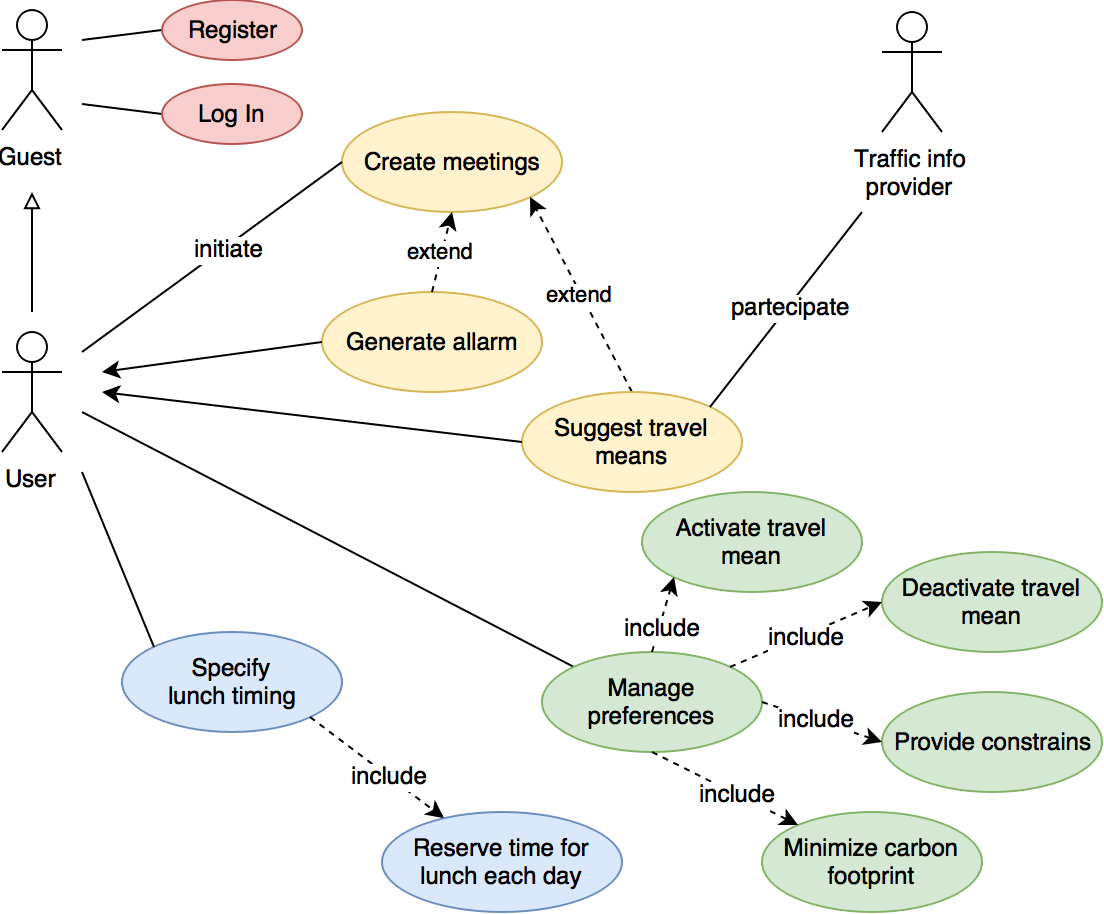
\includegraphics[width=0.75\textwidth]{img/UseCaseModel.png}
		\caption{Use Case Model. Explains actors and functionalities offered by the system.}
		\label{default}
		\end{center}
	\end{figure}
	
	
	\section{User Characteristics}
	The target user is someone who needs an automated system to manage appointments that also handle the scheduling of travels.
	
	The meeting should not overlap with any pre - existing one and should allow the user to move from his/her current position to the meeting position, according with preferred travel means and traffic conditions.
	
	
	\section{Assumptions and Dependences}
	The following assumptions are given for granted:
	\begin{itemize}
	\item  Transport means are complied with the user?s request.
	\item  Device is always connect to the server.
	\item  All users provided correct and valid data at time the registration.
	\item  GPS shows the actual position of the owner.
	\item  Provider Information shows correct and update data.
	\item  The event, when it?s inserted, must not be in the past.
	\end{itemize}
	
	
	\section{Constraints}
	
	
	\subsection{Regulatory policies}
	The application must be allowed by the user to collect his/her position, through GPS.
	
	
	\subsection{Hardware limitations}
	\begin{itemize}
	\item Web application:
		\begin{itemize}
		\item Internet connection
		\item 800x600 screen resolution
		\end{itemize}
	\item Mobile application:
		\begin{itemize}
		\item Internet connection
		\item 50 MB of available storage space
		\item 1GB of RAM
		\item GPS module
		\end{itemize}
	\end{itemize}
	
	
	\subsection{Reliability requirements}
	The system reliability, that is the probability to operate without a failure for a specific period of time, must be at least 99\%.
	
	
	\clearpage
	\section{World and Machine model interpretation}
	In this part of RASD, a description of the system-to-be is provided following the World and Machine model introduced by Jackson and Zave.
	
	\bigskip
	They indicate as the Machine the portion of the system to be developed, typically software ? to ? be plus hardware. The Machine domain is the set of phenomena located entirely in the machine and that the machine control (e.g., machine algorithms, controlled device,?)
	
	\bigskip
	Opposite, the World domain is a set of phenomena that the machine cannot observe.

	\bigskip
	The World is connected with the Machine through Shared Phenomena ? part can be observable both by the Machine and by the World. The Shared Phenomena can be controlled by the world and observed by the Machine or controller by the machine and observe by the world.
	
	\bigskip
	\bigskip
	\begin{figure}[htbp]
		\begin{center}
		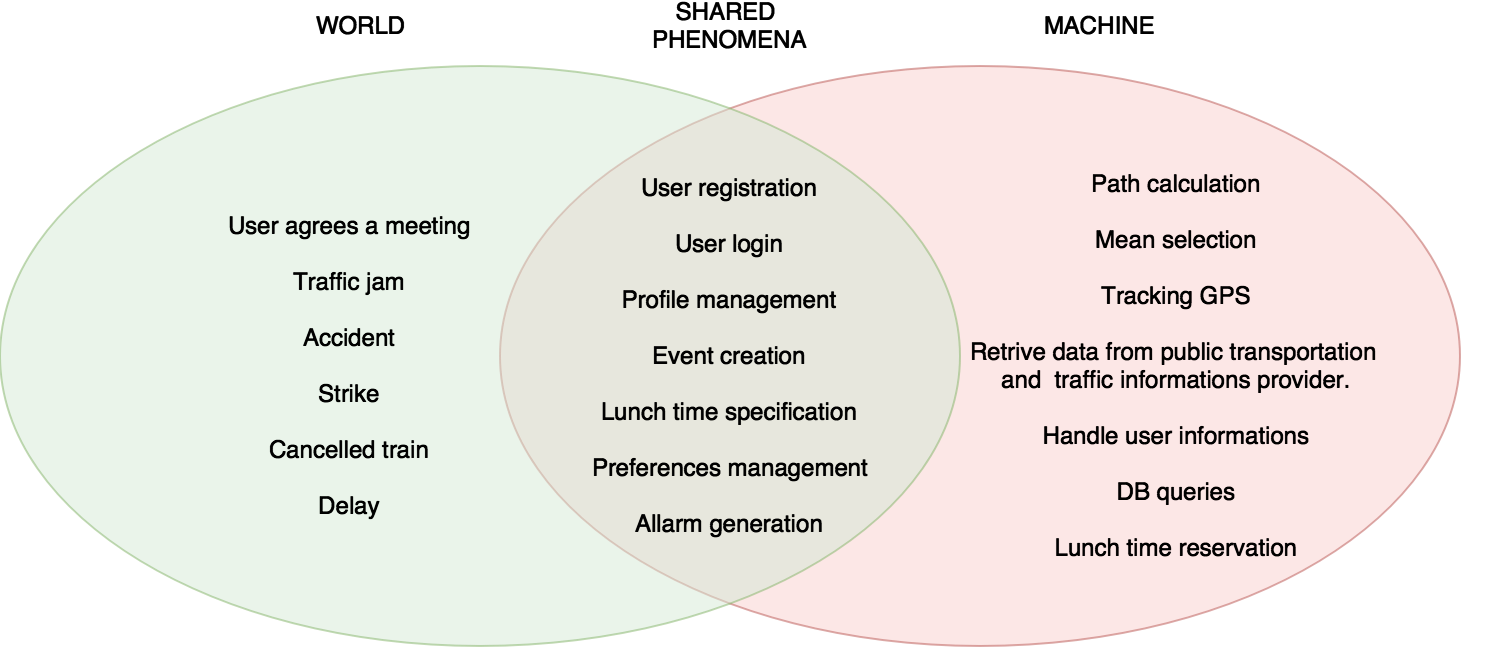
\includegraphics[width=\textwidth]{img/WorldAndMachineModel.png}
		\caption{World and Machine model for the main functionalities offered by the system.}
		\label{default}
		\end{center}
	\end{figure}

	
	\chapter{Specific Requirements}
	Lorem ipsum dolor sit amet, consectetur adipisicing elit, sed do eiusmod
	tempor incididunt ut labore et dolore magna aliqua. Ut enim ad minim veniam,
	quis nostrud exercitation ullamco laboris nisi ut aliquip ex ea commodo
	consequat. Duis aute irure dolor in reprehenderit in voluptate velit esse
	cillum dolore eu fugiat nulla pariatur. Excepteur sint occaecat cupidatat non
	proident, sunt in culpa qui officia deserunt mollit anim id est laborum.
	
	
	\section{External Interface Reqirements}
	Lorem ipsum dolor sit amet, consectetur adipisicing elit, sed do eiusmod
	tempor incididunt ut labore et dolore magna aliqua. Ut enim ad minim veniam,
	quis nostrud exercitation ullamco laboris nisi ut aliquip ex ea commodo
	consequat. Duis aute irure dolor in reprehenderit in voluptate velit esse
	cillum dolore eu fugiat nulla pariatur. Excepteur sint occaecat cupidatat non
	proident, sunt in culpa qui officia deserunt mollit anim id est laborum.
	
	
	\subsection{User Interfaces}
	Lorem ipsum dolor sit amet, consectetur adipisicing elit, sed do eiusmod
	tempor incididunt ut labore et dolore magna aliqua. Ut enim ad minim veniam,
	quis nostrud exercitation ullamco laboris nisi ut aliquip ex ea commodo
	consequat. Duis aute irure dolor in reprehenderit in voluptate velit esse
	cillum dolore eu fugiat nulla pariatur. Excepteur sint occaecat cupidatat non
	proident, sunt in culpa qui officia deserunt mollit anim id est laborum.
	
	
	\subsection{Hardware Interfaces}
	Lorem ipsum dolor sit amet, consectetur adipisicing elit, sed do eiusmod
	tempor incididunt ut labore et dolore magna aliqua. Ut enim ad minim veniam,
	quis nostrud exercitation ullamco laboris nisi ut aliquip ex ea commodo
	consequat. Duis aute irure dolor in reprehenderit in voluptate velit esse
	cillum dolore eu fugiat nulla pariatur. Excepteur sint occaecat cupidatat non
	proident, sunt in culpa qui officia deserunt mollit anim id est laborum.
	
	
	\subsection{Software Interfaces}
	Lorem ipsum dolor sit amet, consectetur adipisicing elit, sed do eiusmod
	tempor incididunt ut labore et dolore magna aliqua. Ut enim ad minim veniam,
	quis nostrud exercitation ullamco laboris nisi ut aliquip ex ea commodo
	consequat. Duis aute irure dolor in reprehenderit in voluptate velit esse
	cillum dolore eu fugiat nulla pariatur. Excepteur sint occaecat cupidatat non
	proident, sunt in culpa qui officia deserunt mollit anim id est laborum.
	
	
	\subsection{Communications Interfaces}
	Lorem ipsum dolor sit amet, consectetur adipisicing elit, sed do eiusmod
	tempor incididunt ut labore et dolore magna aliqua. Ut enim ad minim veniam,
	quis nostrud exercitation ullamco laboris nisi ut aliquip ex ea commodo
	consequat. Duis aute irure dolor in reprehenderit in voluptate velit esse
	cillum dolore eu fugiat nulla pariatur. Excepteur sint occaecat cupidatat non
	proident, sunt in culpa qui officia deserunt mollit anim id est laborum.
	
	
	\section{Functional requirements}
	Lorem ipsum dolor sit amet, consectetur adipisicing elit, sed do eiusmod
	tempor incididunt ut labore et dolore magna aliqua. Ut enim ad minim veniam,
	quis nostrud exercitation ullamco laboris nisi ut aliquip ex ea commodo
	consequat. Duis aute irure dolor in reprehenderit in voluptate velit esse
	cillum dolore eu fugiat nulla pariatur. Excepteur sint occaecat cupidatat non
	proident, sunt in culpa qui officia deserunt mollit anim id est laborum.
	
	
	\section{Performance requiremens}
	Lorem ipsum dolor sit amet, consectetur adipisicing elit, sed do eiusmod
	tempor incididunt ut labore et dolore magna aliqua. Ut enim ad minim veniam,
	quis nostrud exercitation ullamco laboris nisi ut aliquip ex ea commodo
	consequat. Duis aute irure dolor in reprehenderit in voluptate velit esse
	cillum dolore eu fugiat nulla pariatur. Excepteur sint occaecat cupidatat non
	proident, sunt in culpa qui officia deserunt mollit anim id est laborum.
	
	
	\section{Design constrains}
	Lorem ipsum dolor sit amet, consectetur adipisicing elit, sed do eiusmod
	tempor incididunt ut labore et dolore magna aliqua. Ut enim ad minim veniam,
	quis nostrud exercitation ullamco laboris nisi ut aliquip ex ea commodo
	consequat. Duis aute irure dolor in reprehenderit in voluptate velit esse
	cillum dolore eu fugiat nulla pariatur. Excepteur sint occaecat cupidatat non
	proident, sunt in culpa qui officia deserunt mollit anim id est laborum.
	
	
	\subsection{Standards compliance}
	Lorem ipsum dolor sit amet, consectetur adipisicing elit, sed do eiusmod
	tempor incididunt ut labore et dolore magna aliqua. Ut enim ad minim veniam,
	quis nostrud exercitation ullamco laboris nisi ut aliquip ex ea commodo
	consequat. Duis aute irure dolor in reprehenderit in voluptate velit esse
	cillum dolore eu fugiat nulla pariatur. Excepteur sint occaecat cupidatat non
	proident, sunt in culpa qui officia deserunt mollit anim id est laborum.
	
	
	\subsection{Hardware limitations}
	Lorem ipsum dolor sit amet, consectetur adipisicing elit, sed do eiusmod
	tempor incididunt ut labore et dolore magna aliqua. Ut enim ad minim veniam,
	quis nostrud exercitation ullamco laboris nisi ut aliquip ex ea commodo
	consequat. Duis aute irure dolor in reprehenderit in voluptate velit esse
	cillum dolore eu fugiat nulla pariatur. Excepteur sint occaecat cupidatat non
	proident, sunt in culpa qui officia deserunt mollit anim id est laborum.
	
	
	\subsection{Any other constrain}
	Lorem ipsum dolor sit amet, consectetur adipisicing elit, sed do eiusmod
	tempor incididunt ut labore et dolore magna aliqua. Ut enim ad minim veniam,
	quis nostrud exercitation ullamco laboris nisi ut aliquip ex ea commodo
	consequat. Duis aute irure dolor in reprehenderit in voluptate velit esse
	cillum dolore eu fugiat nulla pariatur. Excepteur sint occaecat cupidatat non
	proident, sunt in culpa qui officia deserunt mollit anim id est laborum.
	
	
	\section{Software System Attributes}
	Lorem ipsum dolor sit amet, consectetur adipisicing elit, sed do eiusmod
	tempor incididunt ut labore et dolore magna aliqua. Ut enim ad minim veniam,
	quis nostrud exercitation ullamco laboris nisi ut aliquip ex ea commodo
	consequat. Duis aute irure dolor in reprehenderit in voluptate velit esse
	cillum dolore eu fugiat nulla pariatur. Excepteur sint occaecat cupidatat non
	proident, sunt in culpa qui officia deserunt mollit anim id est laborum.
	
	
	\subsection{Reliability}
	Lorem ipsum dolor sit amet, consectetur adipisicing elit, sed do eiusmod
	tempor incididunt ut labore et dolore magna aliqua. Ut enim ad minim veniam,
	quis nostrud exercitation ullamco laboris nisi ut aliquip ex ea commodo
	consequat. Duis aute irure dolor in reprehenderit in voluptate velit esse
	cillum dolore eu fugiat nulla pariatur. Excepteur sint occaecat cupidatat non
	proident, sunt in culpa qui officia deserunt mollit anim id est laborum.
	
	
	\subsection{Availability}
	Lorem ipsum dolor sit amet, consectetur adipisicing elit, sed do eiusmod
	tempor incididunt ut labore et dolore magna aliqua. Ut enim ad minim veniam,
	quis nostrud exercitation ullamco laboris nisi ut aliquip ex ea commodo
	consequat. Duis aute irure dolor in reprehenderit in voluptate velit esse
	cillum dolore eu fugiat nulla pariatur. Excepteur sint occaecat cupidatat non
	proident, sunt in culpa qui officia deserunt mollit anim id est laborum.
	
	
	\subsection{Security}
	Lorem ipsum dolor sit amet, consectetur adipisicing elit, sed do eiusmod
	tempor incididunt ut labore et dolore magna aliqua. Ut enim ad minim veniam,
	quis nostrud exercitation ullamco laboris nisi ut aliquip ex ea commodo
	consequat. Duis aute irure dolor in reprehenderit in voluptate velit esse
	cillum dolore eu fugiat nulla pariatur. Excepteur sint occaecat cupidatat non
	proident, sunt in culpa qui officia deserunt mollit anim id est laborum.
	
	
	\subsection{Mantainability}
	Lorem ipsum dolor sit amet, consectetur adipisicing elit, sed do eiusmod
	tempor incididunt ut labore et dolore magna aliqua. Ut enim ad minim veniam,
	quis nostrud exercitation ullamco laboris nisi ut aliquip ex ea commodo
	consequat. Duis aute irure dolor in reprehenderit in voluptate velit esse
	cillum dolore eu fugiat nulla pariatur. Excepteur sint occaecat cupidatat non
	proident, sunt in culpa qui officia deserunt mollit anim id est laborum.
	
	
	\subsection{Portability}
	Lorem ipsum dolor sit amet, consectetur adipisicing elit, sed do eiusmod
	tempor incididunt ut labore et dolore magna aliqua. Ut enim ad minim veniam,
	quis nostrud exercitation ullamco laboris nisi ut aliquip ex ea commodo
	consequat. Duis aute irure dolor in reprehenderit in voluptate velit esse
	cillum dolore eu fugiat nulla pariatur. Excepteur sint occaecat cupidatat non
	proident, sunt in culpa qui officia deserunt mollit anim id est laborum.
	
	
	\chapter{Formal Analysis Using Alloy}
	Lorem ipsum dolor sit amet, consectetur adipisicing elit, sed do eiusmod
	tempor incididunt ut labore et dolore magna aliqua. Ut enim ad minim veniam,
	quis nostrud exercitation ullamco laboris nisi ut aliquip ex ea commodo
	consequat. Duis aute irure dolor in reprehenderit in voluptate velit esse
	cillum dolore eu fugiat nulla pariatur. Excepteur sint occaecat cupidatat non
	proident, sunt in culpa qui officia deserunt mollit anim id est laborum.
	
	
	\chapter{Effort Spent}
	Lorem ipsum dolor sit amet, consectetur adipisicing elit, sed do eiusmod
	tempor incididunt ut labore et dolore magna aliqua. Ut enim ad minim veniam,
	quis nostrud exercitation ullamco laboris nisi ut aliquip ex ea commodo
	consequat. Duis aute irure dolor in reprehenderit in voluptate velit esse
	cillum dolore eu fugiat nulla pariatur. Excepteur sint occaecat cupidatat non
	proident, sunt in culpa qui officia deserunt mollit anim id est laborum.
	
	
	\chapter{References}
	Lorem ipsum dolor sit amet, consectetur adipisicing elit, sed do eiusmod
	tempor incididunt ut labore et dolore magna aliqua. Ut enim ad minim veniam,
	quis nostrud exercitation ullamco laboris nisi ut aliquip ex ea commodo
	consequat. Duis aute irure dolor in reprehenderit in voluptate velit esse
	cillum dolore eu fugiat nulla pariatur. Excepteur sint occaecat cupidatat non
	proident, sunt in culpa qui officia deserunt mollit anim id est laborum.
	
\end{document}
